\section{Main Results}

\Cref{tab:cross_model} reports annualized Sharpe ratios for all
(model, feature configuration) combinations on the held-out test set
(weeks 275--323, 49 panel weeks; 48 valid portfolio-return observations
after masking).
Rows correspond to six information sets of increasing richness;
columns span three deep learning architectures and six traditional baselines,
evaluated under both equal-weight (EW) and price-weight (PW) portfolio
construction schemes.

% Auto-generated table — run: python paper/scripts/gen_tables.py
% Auto-generated by gen_tables.py -- do not edit manually
\begin{table*}[t]
\centering
\caption{Cross-model comparison: annualised Sharpe ratios on the test set. The held-out period contains 49 panel weeks; after masking, portfolio metrics use 48 valid weekly long-short returns.}
\label{tab:cross_model}
\begingroup
\footnotesize
\setlength{\tabcolsep}{3pt}
\begin{tabular}{@{}lrrrrrrrrr@{}}
\toprule
\thead{Information Set} & \thead{CS\_Gated} & \thead{LSTM} & \thead{TFT} & \thead{OLS} & \thead{ElasticNet} & \thead{PCA} & \thead{PLS} & \thead{RF} & \thead{GBT} \\
\midrule
\multicolumn{10}{l}{\textit{Panel A: Equal-Weight (EW)}} \\
\midrule
Price{+}Technical & 1.344 & 1.447 & 0.116 & 1.208 & 1.275 & 0.391 & 0.642 & 1.218 & \textbf{1.737} \\
{+}Onchain & \textbf{2.753$^\dagger$} & 1.128 & 1.319 & 1.085 & 1.275 & 0.421 & 0.624 & 1.554 & 1.623 \\
All & 0.856 & 0.366 & 0.442 & 1.194 & 1.275 & 0.457 & 0.624 & \textbf{2.098} & -0.009 \\
{+}Trump & 1.242 & 0.588 & 0.930 & 1.289 & 1.093 & 0.375 & 0.828 & \textbf{1.983} & 1.147 \\
{+}ETF & \textbf{1.421} & 0.574 & 0.885 & 1.194 & 1.275 & 0.457 & 0.624 & 1.272 & -0.009 \\
{+}Trump{+}ETF & 1.824 & \textbf{2.033$^\dagger$} & 1.761 & 1.310 & 1.093 & 0.375 & 0.828 & 1.475 & 1.147 \\
\midrule
\multicolumn{10}{l}{\textit{Panel B: Price-Weighted (PW)}} \\
\midrule
Price{+}Technical & 1.333 & \textbf{2.453$^\dagger$} & 0.135 & 1.130 & 1.275 & 0.434 & 0.578 & 1.289 & 1.563 \\
{+}Onchain & \textbf{2.607$^\dagger$} & 0.932 & 1.059 & 1.003 & 1.275 & 0.464 & 0.870 & 1.471 & 1.434 \\
All & 1.252 & 0.591 & 0.165 & 1.244 & 1.275 & 0.564 & 0.725 & \textbf{1.572$^\dagger$} & 0.998 \\
{+}Trump & 0.895 & 0.566 & 0.977 & 1.314 & 1.028 & 0.409 & 0.815 & \textbf{1.620} & 1.235 \\
{+}ETF & 1.157 & 0.356 & 0.867 & 0.932 & 1.275 & 0.565 & 1.026 & \textbf{1.431} & 0.998 \\
{+}Trump{+}ETF & 1.613 & \textbf{2.135$^\dagger$} & 1.869$^\dagger$ & 1.203 & 1.029 & 0.410 & 0.815 & 1.398 & 1.235 \\
\bottomrule
\end{tabular}
\endgroup
\par\vspace{0.35em}
\begin{minipage}{0.96\linewidth}
\raggedright\footnotesize
\textit{Note:} $\dagger$ indicates that the 95\% circular block-bootstrap confidence interval for the annualised Sharpe ratio excludes zero. Bootstrap block length is $b=\max(2,\lfloor T^{1/3}\rfloor)$. Bold entries mark the best model within each information set and weighting scheme.
\end{minipage}
\end{table*}


\paragraph{CrossSectionalGatedNet.}
CS-Gated achieves the highest single-model Sharpe ratio of 2.75 (EW)
and 2.61 (PW) under the \texttt{+Onchain} configuration, making it the
top-performing model when on-chain fundamentals serve as the primary
feature group.
The absence of temporal encoding is not a handicap in this regime:
on-chain metrics such as NVT and MVRV provide strong contemporaneous
cross-sectional signal—tokens with low NVT relative to their peers are
arguably undervalued regardless of their prior price trajectory—and
the GRN layers learn to exploit these levels without needing historical
context.
In contrast, CS-Gated does not benefit from adding Trump social media or
ETF flow features; performance under \texttt{+Trump+ETF} (SR = 1.82 EW)
falls well below its \texttt{+Onchain} peak and even below LSTM in the
same configuration.
This divergence reveals a key architectural limitation: CS-Gated processes
all features as a single cross-sectional snapshot and cannot distinguish
between structurally persistent signals (on-chain levels) and
event-driven, time-varying signals (tweet counts, ETF flow reversals)
that only carry information in specific weeks.
Its relative strength is therefore narrow but economically interpretable.
Among the six information sets, CS-Gated is the only deep learning model
that clearly dominates both EW and PW in the \texttt{+Onchain} row, and it
also remains competitive in \texttt{+ETF}, especially under EW.
However, once the signal requires sequencing rather than level comparison,
its advantage over both temporal models and Random Forest narrows or
disappears.

\paragraph{LSTM.}
LSTM with \texttt{+Trump+ETF} achieves SR = 2.13 (PW) and 2.03 (EW),
the best configuration among temporal deep learning models.
The pattern is reversed relative to CS-Gated: LSTM degrades when all
macro and on-chain features are added together (\texttt{All}, SR = 0.37 EW),
but recovers strongly when Trump social media and ETF flow series are
included (+1.54 SR delta over \texttt{All} in EW).
The interpretation is that the LSTM encoder extracts temporal patterns
from the social media and ETF time series—such as the sequence of large
inflow days following an ETF approval event, or the clustering of
policy-relevant Trump posts before a regulatory announcement—that are
invisible to a purely cross-sectional architecture operating on
contemporaneous inputs.
This complementarity suggests that CS-Gated and LSTM are not competing
models but rather models specialized for different signal types within
the same universe.
The weighting comparison is also informative.
Under \texttt{Price+Technical}, LSTM reaches SR = 2.45 in PW versus 1.45 in
EW, the best score in that row under PW.
This gap suggests that the recurrent momentum signal is strongest among
larger, more liquid tokens, whereas the equal-weighted universe introduces
more small-cap noise.
By contrast, the weak \texttt{All} result shows that temporal depth by
itself does not solve the problem of mixing predictors with very different
economic horizons.

\paragraph{Temporal Fusion Transformer.}
TFT exhibits the weakest baseline performance among deep learning models,
particularly in the \texttt{Price+Technical} configuration (SR = 0.12 EW,
0.14 PW), likely because the Variable Selection Network overfits to a small
feature set during the training phase, producing unstable gate weights
across seeds.
However, TFT recovers with the \texttt{+Trump+ETF} configuration
(SR = 1.76 EW, 1.87 PW), a delta of +1.72 SR over \texttt{All} (EW)
that mirrors and slightly exceeds the benefit seen in LSTM.
This parallel improvement confirms that the temporal attention mechanism
in both LSTM and TFT is capable of extracting policy-linked time-series
signals; the difference between the two architectures lies in stability
(LSTM has lower per-seed variance; see \Cref{sec:analysis:ensemble})
rather than in their capacity to leverage alternative data.
The full-scale VSN, with $\sim$27K parameters, contributes to this recovery
by providing richer nonlinear per-feature gating, consistent with the
original \citet{lim2021temporal} specification.
Compared directly with LSTM, TFT is relatively better in the intermediate
feature sets where selection among heterogeneous inputs matters more than raw
sequence modeling.
For example, TFT exceeds LSTM in \texttt{+Onchain} and \texttt{+Trump}
under both weighting schemes.
Even so, once the richest event-driven feature set is available
(\texttt{+Trump+ETF}), LSTM still delivers the stronger headline Sharpe,
which is consistent with the view that simpler temporal encoders can be more
stable than heavier attention-based architectures in a short sample.

\paragraph{Traditional baselines.}
Traditional models are competitive and occasionally dominant.
Random Forest achieves SR = 2.10 (EW) and 1.57 (PW) under the
\texttt{All} configuration, outperforming all three deep learning models
in that row.
This result reflects RF's ability to exploit feature interactions via
random splits in high-dimensional feature space without suffering from
the optimization instability that affects DL models when features with
heterogeneous predictive horizons are mixed together.
Gradient Boosting shows more erratic behavior, with SR = $-$0.009 under
\texttt{All} and \texttt{+ETF} (EW)—possibly indicating overfitting to
training-set cross-sectional patterns that do not generalize—while
recovering to SR = 1.15 under \texttt{+Trump+ETF}.
ElasticNet produces a nearly feature-invariant result across the tested
information sets.
Its Sharpe ratio is almost constant across the non-Trump configurations
(about 1.28 under both weighting schemes) and shifts only marginally once the
Trump feature group is included, suggesting that the cross-validated penalty
path collapses onto a narrow, stable subset of predictors and does not exploit
the additional information in the richer feature sets.
OLS is more consistently positive, but its performance ceiling remains below
the leading nonlinear models.
The latent-factor baselines, PCA and PLS, are weaker overall.
Their Sharpe ratios remain well below the leading nonlinear models across
almost every configuration, which suggests that compressing the predictor set
into a small number of common components removes too much token-specific
cross-sectional information.
PLS is occasionally more competitive than PCA under PW, but neither latent
projection method seriously challenges RF, CS-Gated, or the best LSTM
specifications.

\paragraph{Weighting schemes.}
The EW/PW comparison indicates where each model's signal is concentrated.
CS-Gated is comparatively balanced in the on-chain specification
(2.75 EW, 2.61 PW), implying that the valuation signal is present across
the broader cross-section rather than being confined to the largest names.
LSTM shows the sharpest PW advantage in the price-technical and
\texttt{+Trump+ETF} settings, which is consistent with temporal patterns
being easier to exploit in larger, more liquid assets.
Random Forest, by contrast, loses more of its advantage when moving from EW
to PW in the richer feature sets, suggesting that part of its strength comes
from extracting nonlinear interactions among smaller tokens that receive more
weight in equal-weight portfolios.

\paragraph{Overall comparison and take-aways.}
Overall, the results reveal a consistent pattern: no single model
dominates across all feature configurations, and the optimal architecture
depends critically on which signal type is being exploited.
CS-Gated dominates when the feature set is limited to contemporaneous
fundamentals (on-chain levels); LSTM and TFT pull ahead when the
predictive information is embedded in time-series patterns of social
media and ETF flows.
Traditional models—particularly Random Forest—remain formidable
competitors in high-dimensional feature regimes where regularized
non-linearity, rather than temporal depth, is the key inductive bias.
The broader implication is not that deep learning uniformly
dominates traditional methods, but that objective design and
architecture-signal alignment determine when deep learning can
outperform them.

\section{Cumulative Returns}

%insert Figure 1 — combined cumulative returns
\begin{figure}[t]
  \centering
  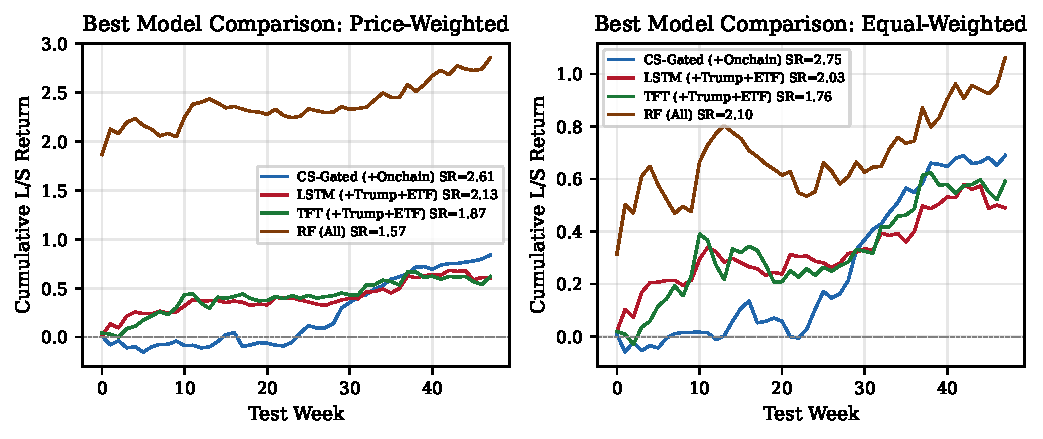
\includegraphics[width=\linewidth]{figures/cum_returns_combined.pdf}
  \caption{Cumulative long-short returns for the best configuration of
           each model (CS-Gated \texttt{+Onchain}, LSTM \texttt{+Trump+ETF},
           TFT \texttt{+Trump+ETF}, and RF \texttt{All}). Legend entries report
           each strategy's terminal cumulative return (CR), i.e.\ the final
           value of the plotted curve; this is a magnitude measure, not the
           risk-adjusted Sharpe ratio of \Cref{fig:sr_combined}.}
  \label{fig:cumret_combined}
\end{figure}

\Cref{fig:cumret_combined} plots the cumulative long-short returns for the
best configuration of the three deep learning models and the best Random
Forest specification.
The figure is broadly consistent with the table-based ranking results:
the strongest specifications separate from zero over the test period, but
they do so through different paths.
RF reaches the largest cumulative level in this figure, especially under
price weighting, but its gains are more episodic and concentrated early in
the test window.
CS-Gated and LSTM accumulate more gradually.
This is consistent with RF's configuration-specific dominance in
\Cref{tab:cross_model} rather than uniform superiority across rows.

%insert Figure — Sharpe ratio comparison
\begin{figure}[t]
  \centering
  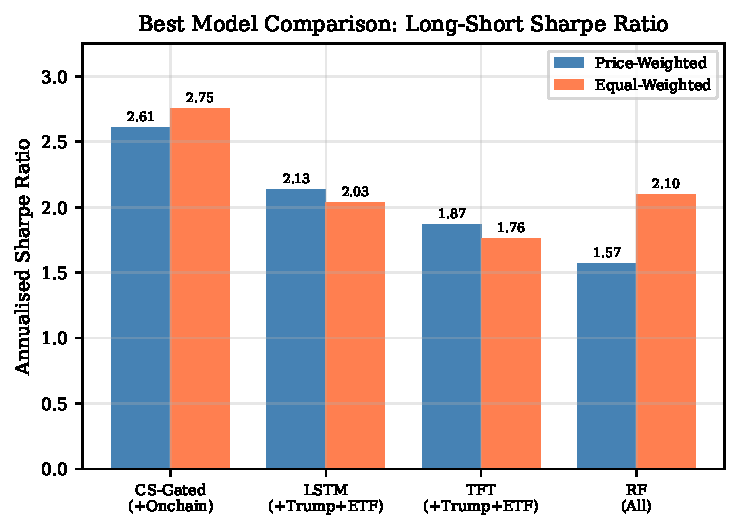
\includegraphics[width=0.8\linewidth]{figures/sr_comparison.pdf}
  \caption{Annualized long-short Sharpe ratios for the best configuration of
           each model (CS-Gated \texttt{+Onchain}, LSTM \texttt{+Trump+ETF},
           TFT \texttt{+Trump+ETF}, and RF \texttt{All}), under price-weighted
           and equal-weighted portfolio construction. Unlike
           \Cref{fig:cumret_combined}, which plots terminal cumulative return,
           this figure reports risk-adjusted performance.}
  \label{fig:sr_combined}
\end{figure}

\Cref{fig:sr_combined} restates the same comparison on a risk-adjusted basis.
CS-Gated (\texttt{+Onchain}) attains the highest Sharpe ratio under both
weighting schemes (2.61 PW, 2.75 EW), whereas Random Forest---despite reaching
the largest cumulative return in \Cref{fig:cumret_combined}---earns the lowest
price-weighted Sharpe ratio (1.57), because its gains are large but volatile.
The two figures therefore measure different objects: cumulative return rewards
total magnitude, while the Sharpe ratio rewards consistency, and it is the
latter that underpins the model ranking in \Cref{tab:cross_model}.

\section{Decile Sharpe Ratios}

\begin{figure}[t]
  \centering
  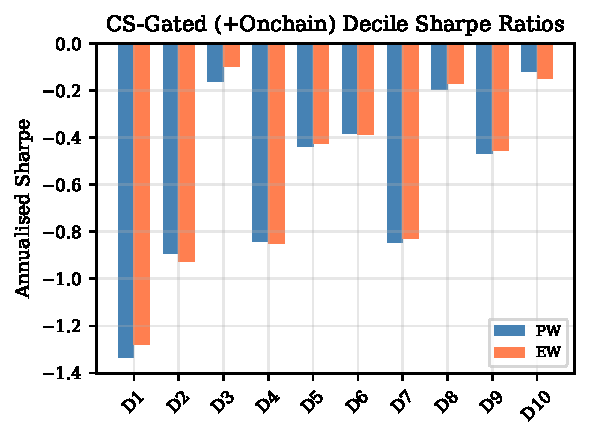
\includegraphics[width=\linewidth]{figures/decile_sharpe_cs_gated.pdf}
  \caption[Decile Sharpe ratios for CS-Gated]{Sharpe ratio of each predicted-rank decile portfolio for
           CS-Gated (\texttt{+Onchain}). Decile 1 corresponds to the
           short leg (lowest predicted rank); decile 10 corresponds to the
           long leg (highest predicted rank). Bars report both PW and EW
           portfolios.}
  \label{fig:decile_cs_gated}
\end{figure}

\Cref{fig:decile_cs_gated} shows the Sharpe ratio of each predicted-rank
decile portfolio for CS-Gated (+Onchain).
The pattern should be interpreted through the long-short spread rather than
as a perfectly monotone decile ladder.
These bars are standalone decile-portfolio Sharpe ratios, whereas
\Cref{tab:cross_model} reports the Sharpe ratio of the D10--D1 long-short
spread; their ordering therefore need not match exactly.
During this test window, several standalone decile portfolios have negative
Sharpe ratios, but the lowest predicted decile performs materially worse than
the highest predicted decile.
The economically relevant result is therefore cross-sectional separation:
the model identifies assets to avoid more strongly than it produces a smooth
ranking across every intermediate bucket.
Middle deciles are noisy, which is unsurprising given only 48 valid weekly
portfolio observations.
